% Preamble
% ---
\documentclass{article}

% Packages
% ---
\usepackage{amsmath} % Advanced math typesetting
\usepackage{amsfonts} % Advanced math typesetting
\usepackage{amssymb} % More Math
\usepackage[utf8]{inputenc} % Unicode support (Umlauts etc.)
\usepackage[ngerman]{babel} % Change hyphenation rules
\usepackage{hyperref} % Add a link to your document
\usepackage{graphicx} % Add pictures to your document
\usepackage{listings} % Source code formatting and highlighting
\usepackage{booktabs}

\DeclareMathOperator*{\argmax}{arg\,max}


% Title
%---
\title{Optimizing Weighted Lower Linear Envelope Potentials Within Latent-SVM Framework}
\author{Chang Li}
\date{\today}

% Document
%---
\begin{document}
	\maketitle
	
	\section{Introduction}
	One interesting task in machine learning is labeling over complex and structured objects. Many applications such as image segmentation, motif finding and noun-phrase parsing involved with representing jointly correlated variables. Algorithm frameworks like Markov Random Field (MRF) containing higher order energy functions and max margin method for Structural SVM are raising interests recently due to their capability of representing structural dependencies of variables and ensuring computationally feasible approximate or exact inference. \\
	Higher order potentials can be optimized efficiently using modern Linear Programming frameworks. For example, Kohli and Kumar\cite{kohli2009robust} developed lower linear envelope potentials by introducing auxiliary variables to reduce the potential function to a pairwise formulation. Thus the formulation can be optimized using LP programming. However, they only provide an approximate routine for the problem.\\ Another powerful algorithm called “graph-cuts” which can do exact inference on binary MRFs with internal submodular potentials was well studied in past years. Gould\cite{gouldlearning} extended the previous research via graph-cuts to do an exact inference using weighted lower linear envelope potentials and optimized the model parameters within a max-margin learning framework. However, the approximation used in their work using a fixed spaced break-points lower linear envelope. If the equally spaced constraint can be removed, their formulation will result in a latent SVM.\\
	In practical, many information providing useful cues for prediction is not directly observable from data. For motif (repeated patterns in DNA sequences) finding problem, as an example, the task is to find motifs from a set of DNA sequences where the location of these motifs are unknown. Thus the information of position can be treated as hidden variable and is important to be considered in the model. Issues like this have been studied by many researchers and latent SVMs, which can explicitly model hidden variables with joint feature vectors, outperforms many other methods. \\
	The latent SVM was developed by Felzenszwalb et al.\cite{felzenszwalb2008discriminatively} and Yu and Joachims\cite{yu2009learning} independently in different ways. The main idea is introducing a latent variable to extend the feature vector, which results in a generalized user defined loss function, e.g. Hinge Loss, with an upper bound. Then the optimization was done by using Concave-Convex Procedure (CCCP) algorithm.\\
	In this project, our goal is to study the relationship between the algorithm proposed in \cite{gouldlearning} and latent SVM framework. The main challenge is how to relax the fixed space constraint and find an auxiliary variable independent approximation of the lower linear envelope. We will experiment our algorithm on Weizmann Horse dataset\cite{borenstein2002class}\cite{borenstein2008combined}. Other extensions may also be studied, e.g. extending the loss function\cite{pletscher2012learning}.

	\section{Literature Review}
	Learning structural objects from unknown probability distribution is becoming popular in recent years. Tsochantaridis et al.\cite{tsochantaridis2005large} generalized multiclass SVMs\cite{crammer2002algorithmic} to structural SVMs by extending feature vectors to joint feature vectors which map features extracted jointly over input-output pairs to discrete output. The exact maximum a posteriori (MAP) problem thus becomes an NP-hard problem. They overcome this by using a method called “Soft-Margin Maximization” and found an upper bound of the loss function.\\
	Based on the previous research, Yu and Joachims\cite{yu2009learning} developed latent SVM by introducing a hidden variable into the joint feature vector. They observed a fact that in real world applications hidden variables are usually intermediate results and are not required as an output. With this fact they followed “Soft-Margin” method and found an upper bound for the loss function with latent variables. However, the resulted object function is still non-convex.\\
	Yuille and Rangarajan \cite{yuille2002concave} developed the Concave-Convex Procedure (CCCP) which is guaranteed to find a local minimum for a Difference-Convex (DC) program. Yu and Joachims\cite{yu2009learning} combined CCCP algorithm by writing their non-convex object function into a difference of two convex function and came up with a EM like 2 steps optimizing algorithm. For each iteration, they first compute latent variables utilizing current parameter vectors and then in turn optimizing parameter vectors using the standard Structural SVM algorithm with previously computed latent variables. \\
	Higher order potentials are raising interests due to their capability to represent dependencies between complex objects. Kohli and Kumar\cite{kohli2009robust} proposed a method to represent a class of higher order potentials with lower (upper) linear envelope potentials. By introducing auxiliary variables, they reduced the linear representation to a pairwise form and proposed an approximate algorithm with standard LP program methods. Following their routine, Gould\cite{gouldlearning} extended their method to a weighted lower linear envelope in binary Markov Random Fields (MRF) which can be solved with an efficient algorithm. They showed the energy function with auxiliary variables is submodular by transforming it into a quadratic pseudo-Boolean form and how “graph-cuts” like algorithm can be applied to do exact inference. They then optimized the model’s parameters under the max margin framework\cite{tsochantaridis2005large}. \\
	In their work they pointed out the potential relationship between their auxiliary representation and latent SVM\cite{yu2009learning}. However, since removing of their fixed space constraint will result dependence between latent variable and parameters, further research still remains open.
	
	\section{Proposal}
	
	\subsection{Theoretical Background}
	In this section, we first briefly introduce how latent SVM is developed\cite{yu2009learning} from standard structural SVMs and how to do "loss-augmented" inference on loss function with latent variables. We then show the fixed space constraint Gould\cite{gouldlearning} use to sample energy function with weighted linear lower envelope potentials and how that formulation is optimized under max margin framework. The relationship between them is studied in the next section.
		\subsubsection{Structural SVMs with latent variables}
		To include unobserved information in the model, Yu\cite{yu2009learning} extended the joint feature function  $\Psi(\mathbf{x},\mathbf{y}) $ with a latent variable $\mathbf{h}\in \mathcal{H}$ to $\Psi(\mathbf{x},\mathbf{y},\mathbf{h}) $. So the inference problem becomes
		$$
		f_w(x) = \argmax_{(\mathbf{y} \times \mathbf{h}) \in \mathcal{Y} \times \mathcal{H}} w\cdot\Psi(\mathbf{x},\mathbf{y},\mathbf{h})
		$$
		Accordingly, the loss function can be extended as
		$$
		\Delta((\mathbf{y}_i,\mathbf{h}^*_i(w)),(\mathbf{\hat{y}}_i(w),\mathbf{\hat{h}}_i(w)))
		$$
		where
		$$
		\mathbf{h}^*_i(w) = \argmax_{\mathbf{h} \in \mathcal{H}} w \cdot \Psi(\mathbf{x}_i,\mathbf{y}_i,\mathbf{h})
		$$
		$$
		(\mathbf{\hat{y}}_i(w),\mathbf{\hat{h}}_i(w))=\argmax_{(\mathbf{y} \times \mathbf{h}) \in \mathcal{Y} \times \mathcal{H}} w\cdot\Psi(\mathbf{x}_i,\mathbf{y},\mathbf{h})
		$$
		However, this formulation of loss function can not be applied ``loss-augmented inference'' because the dependece on $\mathbf{h}^*_i(w)$ of the ground truth variable $y_i$.  Yu\cite{yu2009learning} argued that the in real world applications, $\mathbf{h}^*_i(w)$ is usually an intermediate result and is not required as an output. And their work focus on the case when
		$$
		\Delta((\mathbf{y}_i,\mathbf{h}^*_i(w)),(\mathbf{\hat{y}}_i(w),\mathbf{\hat{h}}_i(w)))=\Delta(\mathbf{y}_i,\mathbf{\hat{y}}_i(w),\mathbf{\hat{h}}_i(w))
		$$
		The ``loss-augmented inference'' of this formulation can be done as:
		\begin{align*}
			\Delta((\mathbf{y}_i,\mathbf{h}^*_i(w)),(\mathbf{\hat{y}}_i(w),\mathbf{\hat{h}}_i(w)))
			&\leq\\
			&\bigg(\max_{(\mathbf{\hat{y}} \times \mathbf{\hat{h}}) \in \mathcal{Y} \times \mathcal{H}} [w\cdot\Psi(\mathbf{x}_i,\mathbf{\hat{y}},\mathbf{\hat{h}}) + \Delta(\mathbf{y}_i,\mathbf{\hat{y}},\mathbf{\hat{h}})]\bigg)\\
			&-\max_{\mathbf{h} \in \mathcal{H}} w \cdot \Psi(\mathbf{x}_i,\mathbf{y}_i,\mathbf{h})
		\end{align*}
		Hence the optimization problem for Structural SVMs with latent variables can be writen as a difference-convex formulation:
		\begin{align*}
			\min_w\bigg[\frac{1}{2}\|w\|^2+
			C\sum_{i=1}^{n}\big(\max_{(\mathbf{\hat{y}} \times \mathbf{\hat{h}}) \in \mathcal{Y} \times \mathcal{H}} [w\cdot\Psi(\mathbf{x}_i,\mathbf{\hat{y}},\mathbf{\hat{h}}) + \Delta(\mathbf{y}_i,\mathbf{\hat{y}},\mathbf{\hat{h}})]\big)\bigg]\\
			-\bigg[C\sum_{i=1}^{n}\big(\max_{\mathbf{h} \in \mathcal{H}} w \cdot \Psi(\mathbf{x}_i,\mathbf{y}_i,\mathbf{h})\big)\bigg]
		\end{align*}
		which is the difference of two convex functions and can be solved using CCCP\cite{yuille2002concave} algorithm.

		\subsubsection{Weighted Lower Linear Envelope and Large Margin Optimization}
		Suppose we have a binary MRFs $\mathbf{y}=\{y_1,\dots,y_n\}$, $y_i\in\{0,1\}$. A higher-order potential $\psi_c^H(\mathbf{y}_c)$ is an arbitrary function defined on cliques $\mathbf{y}_c=\{y_i : i\in c\}$ where $c\subseteq\{1,\dots,n\}$. Gould\cite{gouldlearning} proposed a weighted lower linear envelope potential as a minimum over a piecewise set of linear functions
		\begin{align}
		\psi_c^H(\mathbf{y}_c) \triangleq \min_{k=1,\dots,K}\bigg\{a_kW_c(\mathbf{y}_c)+b_k\bigg\}
		\end{align}
		where $(a_k,b_k)\in\mathbb{R}^2$ are linear function parameters and
		$$
		W_c(\mathbf{y}_c) = \sum_{i\in c}^{}w_i^cy_i
		$$
		where c is a clique. $w_i^c$ is a per-variable non-negative weight for every nodes in each clique and satisfies $\sum_ {i\in c}^{}w_i^c=1$. Thus $W_c(\mathbf{y}_c) \in [0,1]$.\\\\
		Gould\cite{gouldlearning} reparameterized the potential by sampling $K$ break points uniformly distributed on $[0,1]$. Let linear parameter vector $\boldsymbol{\theta}\in\mathbb{R}^K$ be the sampled values, the energy function satisfying all propositions in \cite{gouldlearning} can be writen as the multiplication of
		\begin{equation*}
		\theta_k = \left\{
		\begin{aligned}
		& b_1	& \text{for} \ k=0\\
		& a_1 & \text{for}\ k=1\\
		& a_{k-1}-a_k  & \text{for} \ k=2,\dots,K\\
		\end{aligned}
		\right.
		\end{equation*}
		where $b_{k+1}=(a_k-a_{k+1})\frac{k}{K}+b_k$, and
		\begin{equation*}
		\phi_k = \left\{
		\begin{aligned}
		& 1	& \text{for} \ k=0\\
		& W(\mathbf{y}) & \text{for}\ k=1\\
		& \bigg(\frac{k-1}{K}-W(\mathbf{y}) \bigg)\bigg[\bigg[ W(\mathbf{y}) > \frac{k-1}{K}\bigg]\bigg]  & \text{for} \ k=2,\dots,K\\
		\end{aligned}
		\right.
		\end{equation*}
		where $\boldsymbol{\phi}(\mathbf{y})\in \mathbb{R}^K$ is the corresponding feature map. Thus we can rewrite the Equation 1 into a linear form
		\begin{align}
		E(\mathbf{y}_c)=\boldsymbol{\theta}^T\boldsymbol{\phi}(\mathbf{y})
		\end{align}
		with constraint $ D\boldsymbol{\theta}\geq \mathbf{0}$ to ensure the concavity. Equation 2 can be optimized using max-margin framework.
		

	\subsection{Extensions}
	
	The main goal of our project is to study the relationship between latent SVM and MRF with higher potentials. As mentioned above, since $b_k$ is a function of $a_k$ and we can retrieve auxiliary vector $\mathbf{z}$ given labels vector $\mathbf{y}$, the object function can be treated as a latent SVM if we could remove the equally spaced constraint.  Challenges remains are how to re-parameterized the energy function without fixed space constraint and solving the non-convex formulation. \\
	We plan to implement our algorithm using MATLAB and Python language. Many existing efficient packages including Latent SVM-struct\cite{yu2009learning} and SVM-struct\cite{tsochantaridis2005large} may be used in our implementation. Our algorithm will be tested on Weizmann Horse dataset\cite{borenstein2002class}\cite{borenstein2008combined}.\\
	Other interesting possible extensions including but not limited to extending loss function, parallel inference using dual decomposition and another generalized potentials might also be studied. Since in \cite{gouldlearning} only consistency constraint is considered (using Hamming Loss), Pletscher\cite{pletscher2012learning} proposed a more sophisticated loss function to encode  higher order statistics. 
	A parallel training algorithm was explored\cite{komodakis2014framework} by utilizing dual decomposition principle to do exact loss-augmented inference within a max-margin learning framework.
	 Li\cite{li2013exploring} proposed a general class of high order potential called Compositional High Order Pattern Potentials (CHOPPs) which can be optimized using standard algorithm for Restricted Boltzmann Machines (RBMs).\\
	 
	\section{Milestones}
	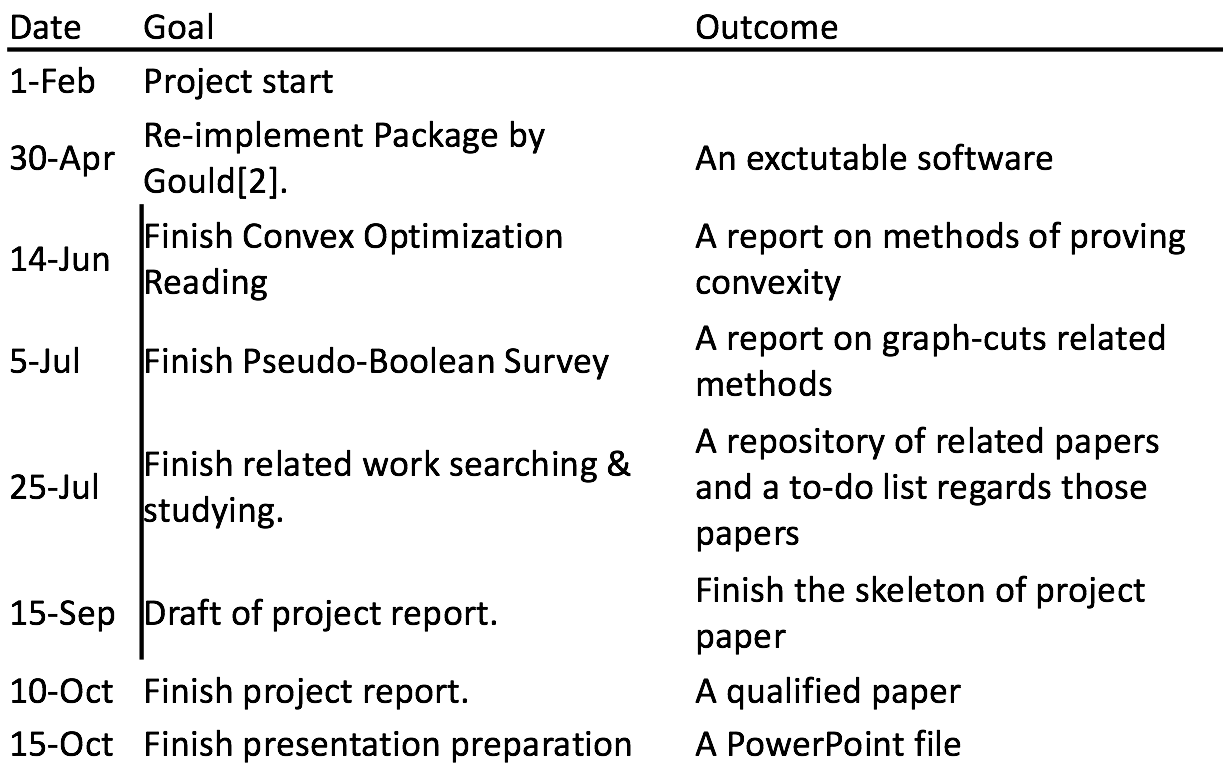
\includegraphics[scale = 0.6]{milestones.png}
	
	
	\renewcommand\refname{Bibliography}
	\bibliographystyle{ieeetr}
	\bibliography{draft}
\end{document}